\documentclass[a4paper]{article}
\usepackage{geometry}
 \geometry{
 a4paper,
 total={170mm,257mm},
 left=20mm,
 top=20mm,
 }
\usepackage[utf8]{inputenc}
\usepackage{amsmath}
\usepackage{amsfonts}
\usepackage{amssymb}
\usepackage[x11names]{xcolor}
\usepackage{hyperref}
\usepackage{graphicx}
\usepackage{subcaption}
\usepackage[many]{tcolorbox}
\usepackage{fontawesome5}



\begin{document}
    \newtcolorbox[]{optionalbox}[1][]{%
        breakable,
        enhanced,
        colback=Green4!5!white,
        colframe=Green4!75!black,
        fonttitle=\bfseries,
        title={Optional part implemented in \texttt{MsMergeSequential} function} %
    }

    \title{OpenMP Mergesort}
    \author{
        \begin{tabular}{@{} l l @{}}
            Alberto Ondei & 11098067 \\
            Abdullah Javed & 10764782 \\
            Andrea Valentini & 11010856
        \end{tabular}
    }
    \maketitle

    \section{Experimental setup}

    The setups used for this project are the following:
    \begin{itemize}
        \item Mi NoteBook Pro, Intel Core i5-8250U 1,6 GHz (4 cores, 8 threads), SDRAM DDR4-2200 of 8 GB.

        \item HP Pavilion - 15, Intel Core i7-8750H 2,2 GHz (6 cores, 12 threads), SDRAM DDR4-2666 of 16 GB.
        
        \item Lenovo Yoga Slim 7, Intel Core Ultra 7 155H (16 cores, 22 threads), LPDDR5x-SDRAM-7467 of 32 GB.
    \end{itemize}
    All notebooks have Ubuntu 24.04 (native) as operating system. The IDE used to develop the project was CLion, but at the very beginning it is also used Visual Studio Code. The CLion IDE, guarantee a very user friendly interface to make some tests and debugs. The project has been divided into some tasks to guarantee each team member to collaborate on the project.

    \section{Performance measurements}

    The tests were conducted on each team member's machine. The reason for this is that the intention was to get a variety of results on very different machines, with different numbers of threads (and frequencies).
    \begin{figure}[!htp]
        \centering
        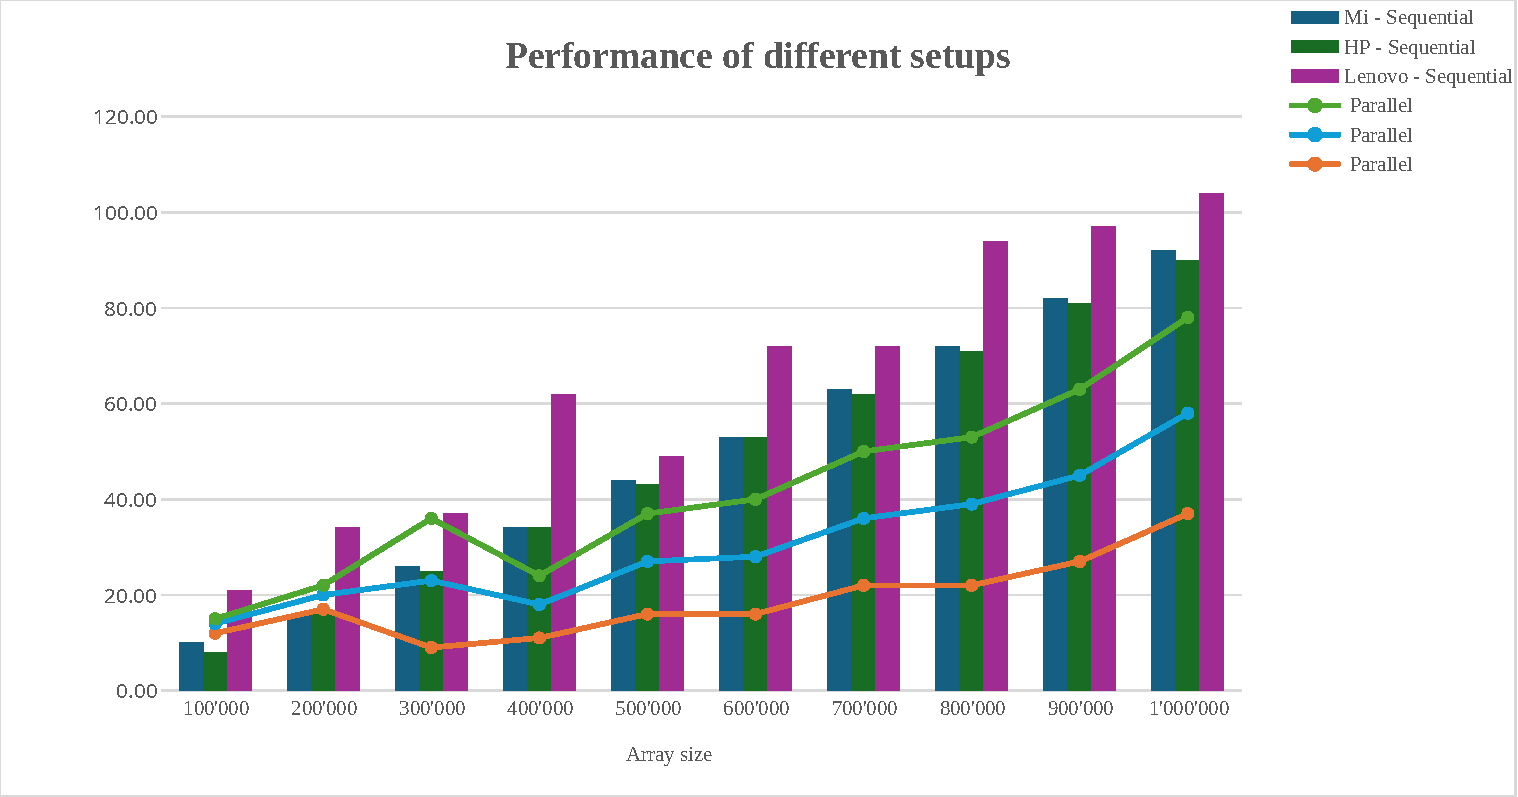
\includegraphics[width=.92\textwidth]{../benchmark/different-setup-benchmark.pdf}
        \caption{Performance of different setups. The \emph{y-axis} indicates the milliseconds required to perform the merge sort, and the \emph{x-axis} indicates the size of the input array. The vertical lines show the milliseconds used by the sequential algorithm on each machine; the horizontal lines show the parallel execution. The execution is almost the same on each different setup, and the gain of the parallel merge sort is not so much for relatively small arrays.}
    \end{figure}

    \noindent
    After taking some measurements on each machine, the team decides to run some benchmarks on one of the setups (HP Pavilion - 15). The following figure shows an interesting result that highlights how much the parallel speedup is soo important with large array size.

    \begin{figure}[!htp]
        \centering
        \begin{subfigure}{.46\textwidth}
            \centering
            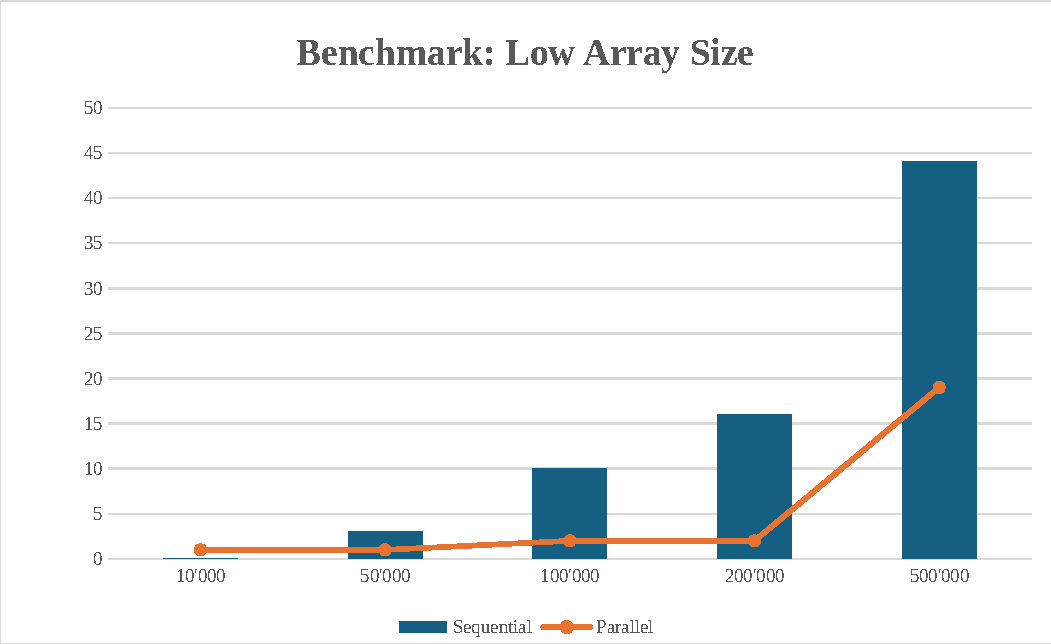
\includegraphics[width=\textwidth]{../benchmark/benchmark-low-array-size.pdf}
        \end{subfigure}
        \begin{subfigure}{.50\textwidth}
            \centering
            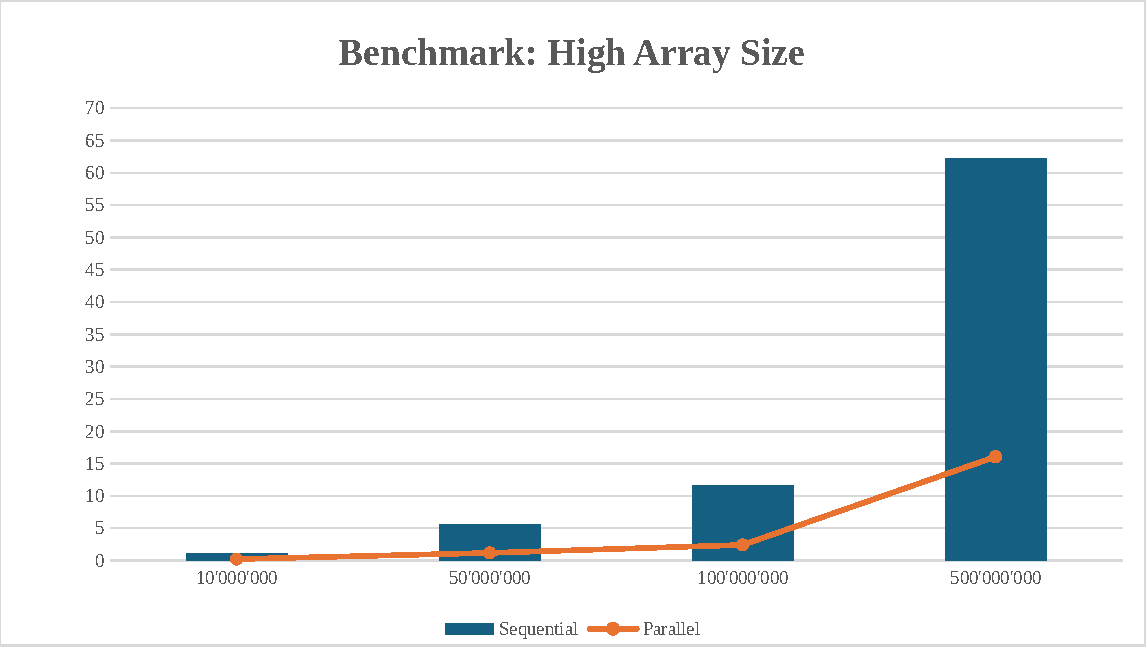
\includegraphics[width=\textwidth]{../benchmark/benchmark-high-array-size.pdf}
        \end{subfigure}
        \caption{In the left figure, the \emph{y-axis} indicates the milliseconds required to perform the merge sort, and the \emph{x-axis} indicates the size of the input array. It shows how the parallel merge sort algorithm suffers from overhead at very small array sizes. Even with a dimension of 10'000, the parallel algorithm is worse than the sequential one (not so much). However, as the size increases, the parallel algorithm takes an important step away from the sequential version. This is especially evident in the right figure. Here the \emph{y-axis} indicates the seconds. When the array size becomes very large, say five hundred million, the parallel algorithm takes only 16 seconds against 63 for the sequential algorithm. Then the speedup of the parallel algorithm is about 4 (63 $\div$ 16).}
    \end{figure}

    \section{Explanation of design choices}
    
    Each recursive call to the \texttt{MsParallel} function generates two tasks: one for sorting the first half and one for the second half. To ensure efficient use of system resources, task creation is controlled by the recursion depth.

    To decide how far to divide the work into parallel tasks, it calculates the optimal depth using the base two logarithm of the total number of available threads to get the best result using hardware parallelism. This approach ensures that the number of tasks created is approximately equal to the number of threads available; creating additional tasks would increase execution time. The size of the array was also taken into account: if the size of the array falls below a certain threshold (called \emph{cut-off} and set to 10'000 elements), sorting continues in a sequential manner. This decision was made to avoid the overhead of managing threads for too small portions of arrays, where parallelism does not offer significant benefits.

    After the parallel tasks for sorting the two halves are completed, it is important to synchronize the threads before proceeding with the merge. The choice to use \texttt{\#pragma omp taskwait} is to ensure that both halves of the array are completely sorted before the merge step is performed.

    \begin{optionalbox}
        In the merge phase, it uses the depth of recursion to decide whether to perform the operation sequentially or in parallel. As it has been done with the \texttt{MsParallel} function, the \texttt{depth} value is used to understand whether to use parallel or sequential technique. If the \texttt{depth} is:
        \begin{itemize}
            \item Less than or equal to zero, the merge is performed sequentially;
            \item Otherwise, the array is split and the algorithm becomes \emph{parallel}. First, it calculates the index of the middle position \texttt{mid1} of the first sub-array. Using the native C++ function \texttt{upper\_bound}, it finds the first element in the second sub-array that is just greater than the \texttt{mid1} value of the first sub-array. This gives the midpoint of the second sub-array \texttt{mid2}. At this point, it creates two parallel tasks:
            \begin{enumerate}
                \item The first task merges the first half of the first sub-array with the part of the second sub-array up to \texttt{mid2}.
                \item The second task merges the second half of the first sub-array with the remaining part of the second sub-array, starting at index \texttt{mid2}.
            \end{enumerate}
            Finally, the \texttt{taskwait} directive is used to wait for the termination of both tasks.
        \end{itemize}
    \end{optionalbox}
    \noindent
    \textcolor{Red3}{\faIcon{exclamation-triangle} \textbf{Disclaimer}} The team tried to implement \texttt{MsMergeSequential} to find an intelligent solution to use both cut-off and parallel techniques. The function was implemented using overloading, so if the \texttt{depth} value is also passed, the parallel version is invoked, otherwise the sequential version is used.
\end{document}
